\chapter{Behoud van massa en kloppende reactievergelijkingen}\label{ch:g8:balanced-equations}

Een houtblok van twee kilo verbrandt in een open haard. 's Ochtends ligt
er nog een paar tientallen gram grijze as. Is er in één nacht bijna twee
kilo materie verdwenen? Eeuwenlang kon niemand dat zeggen. Het antwoord
kwam van een scheikundige die besloot alles te wegen --- ook de gassen
waar niemand ooit aan had gedacht ze te wegen.

\begin{recall}
Bij een \omterm{def:g7:chemical-reactions:reaction}{chemische reactie} worden de \omterm{def:g7:chemical-reactions:reactant}{beginstoffen} verbruikt en de
\omterm{def:g7:chemical-reactions:reactant}{reactieproducten} gevormd; de \omterm{def:g7:atoms-and-molecules:atom}{atomen} van de \omterm{def:g7:chemical-reactions:reactant}{beginstoffen} worden herschikt
tot de \omterm{def:g7:chemical-reactions:reactant}{reactieproducten}, zonder dat er \omterm{def:g7:atoms-and-molecules:atom}{atomen} ontstaan of verdwijnen
(\cref{ch:g7:chemical-reactions}). Een \omterm{def:g7:atoms-and-molecules:formula}{chemische formule} zoals \ce{H2O}
somt de \omterm{def:g7:atoms-and-molecules:atom}{atomen} van een \omterm{def:g7:atoms-and-molecules:molecule}{molecuul} op; een getal ervoor, zoals in
\ce{3H2O}, telt \omterm{def:g7:atoms-and-molecules:molecule}{moleculen} (\cref{ch:g7:atoms-and-molecules}).
\end{recall}

\begin{omfigure}
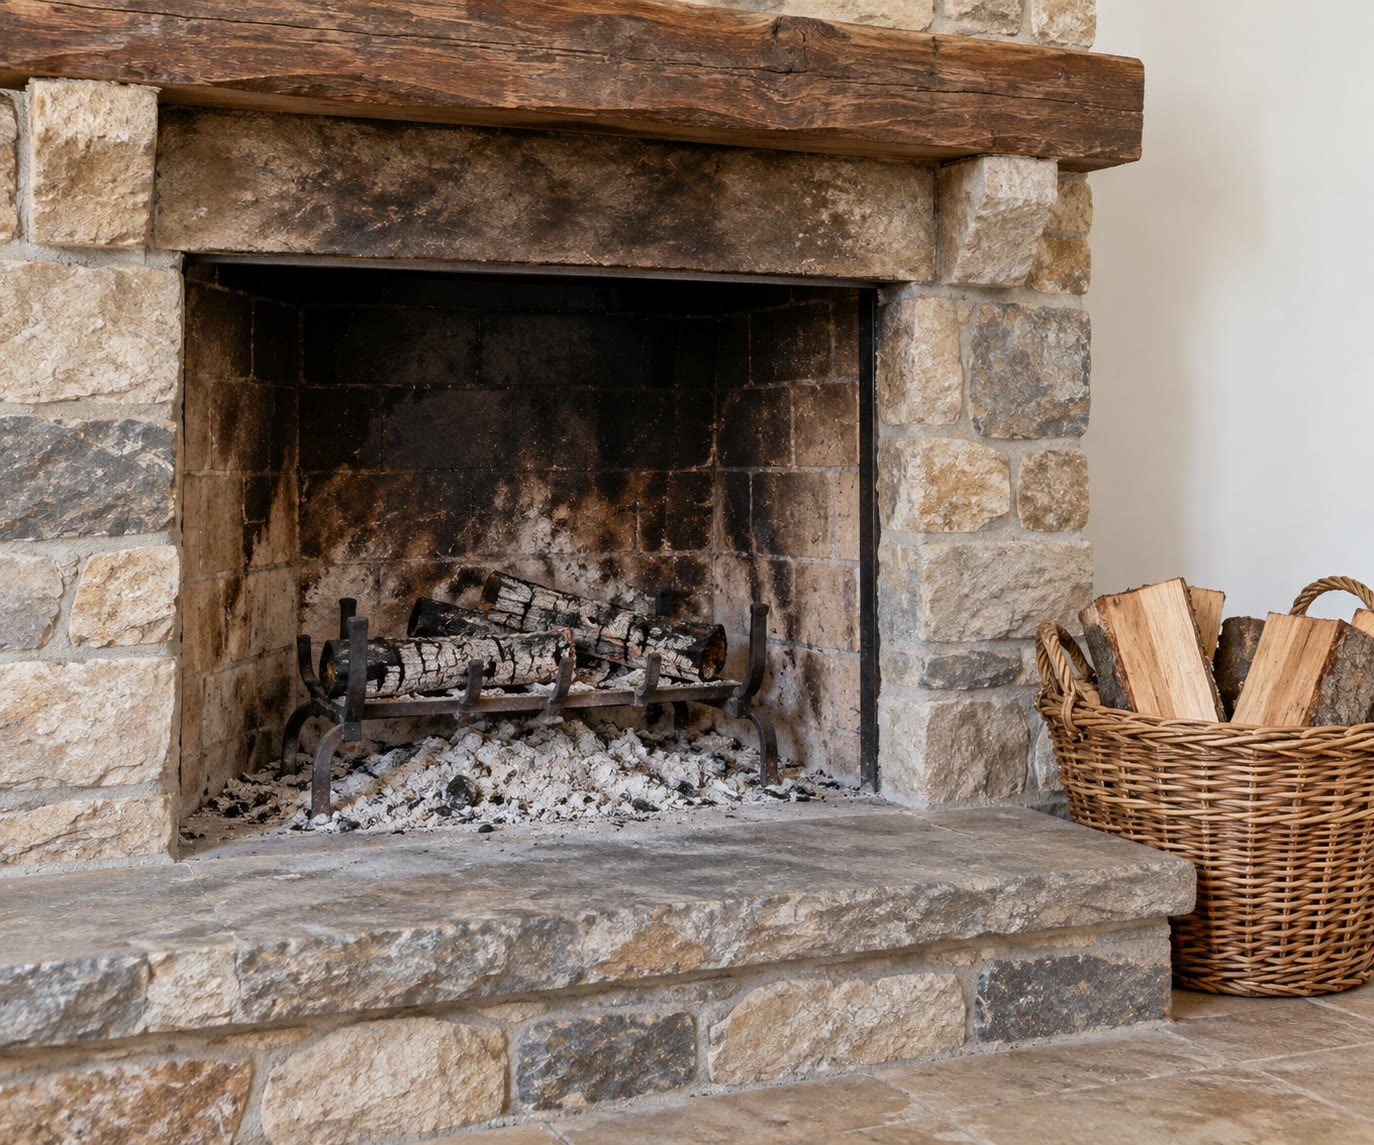
\includegraphics[width=0.5\linewidth]{images/book1/ai/g8-fireplace-ash.jpg}

{\small Een open haard de ochtend erna: een beetje as is alles wat er
van de blokken over is.}
\end{omfigure}

\section{Massa blijft behouden}

\begin{inthelab}[Een reactie wegen in een gesloten kolf]
De docent doet wat azijn in een kolf en baksoda in een ballon die over
de hals is getrokken, en zet het geheel op een balans: \qty{212.4}{g}.
De ballon wordt opgetild zodat de soda in de azijn valt: het \omterm{def:g6:pure-substances-and-mixtures:mixture}{mengsel}
bruist en de ballon zwelt op door het gas dat ontstaat. De balans wijst
nog steeds \qty{212.4}{g} aan. Dezelfde reactie in een open kolf, zonder
ballon, ``verliest'' massa: het gas ontsnapt in het lokaal.
\end{inthelab}

\begin{omfigure}
\begin{tikzpicture}[font=\small, scale=1.15]
  % closed flask
  \pic[transform shape] at (0,0) {balance};
  \pic[transform shape] at (0,0.8) {erlenmeyer={0.25}{omWater!80}};
  \fill[red!55, draw=red!60!black] (0,4.05) ellipse (0.5 and 0.62);
  \fill[red!55] (-0.3,3.45) rectangle (0.3,3.6);
  \node[anchor=north, align=center] at (0,-0.1) {gesloten: het gas blijft\\ in de ballon};
  \node[anchor=west, font=\footnotesize] at (1.25,0.3) {\qty{212.4}{g}};
  % open flask
  \pic[transform shape] at (4,0) {balance};
  \pic[transform shape] at (4,0.8) {erlenmeyer={0.25}{omWater!80}};
  \foreach \y in {3.6,3.95,4.3} \draw[->, black!45, decorate,
    decoration={snake, amplitude=0.6pt, segment length=4pt}] (4,\y) -- (4,\y+0.3);
  \node[anchor=north, align=center] at (4,-0.1) {open: het gas ontsnapt,\\ de aflezing daalt};
  \node[anchor=west, font=\footnotesize] at (5.25,0.3) {\qty{211.9}{g}};
\end{tikzpicture}

{\small Dezelfde reactie, gewogen. In de gesloten kolf verandert de
massa niet; in de open kolf ontsnapt het gas en wijst de balans minder
aan.}
\end{omfigure}

\begin{definition}[Behoud van massa]\label{def:g8:balanced-equations:conservation}
\emph{Behoud van massa}\index{behoud van massa} is de wet die zegt dat
bij een \omterm{def:g7:chemical-reactions:reaction}{chemische reactie} de totale massa van de gevormde
\omterm{def:g7:chemical-reactions:reactant}{reactieproducten} gelijk is aan de totale massa van de verbruikte
\omterm{def:g7:chemical-reactions:reactant}{beginstoffen}. Er gaat niets verloren en er wordt niets gemaakt; materie
verandert alleen van vorm.
\end{definition}

\begin{example}[Het houtblok, goed gewogen]\label{ex:g8:balanced-equations:log}
Als je het brandende houtblok en de zuurstof die het uit de \omterm{def:g4:air-a-mixture-of-gases:air}{lucht}
haalde vooraf kon wegen, en de as, het koolstofdioxide en de waterdamp
achteraf, zouden de twee totalen gelijk zijn. De as is licht omdat de
meeste \omterm{def:g7:chemical-reactions:reactant}{reactieproducten} gassen zijn die door de schoorsteen verdwijnen.
\end{example}

\begin{history}[Lavoisier weegt alles, jaren 1770--1789]
Antoine-Laurent Lavoisier maakte er een regel van om elke stof voor en
na elke reactie te wegen, in afgesloten vaten zodat er geen gas kon
ontsnappen of binnenkomen. Hij liet zien dat metalen zwaarder worden als
ze roesten of \omterm{def:g4:what-a-fire-needs:burning}{verbranden}, doordat ze iets uit de \omterm{def:g4:air-a-mixture-of-gases:air}{lucht} opnemen ---
zuurstof, waaraan hij de naam gaf --- en hij stelde in 1789 dat er bij een
reactie niets ontstaat en niets verloren gaat. Zijn vrouw, Marie-Anne
Paulze Lavoisier, werkte naast hem, legde de experimenten vast en
tekende de apparatuur voor zijn boek.
\end{history}

\begin{omfigure}
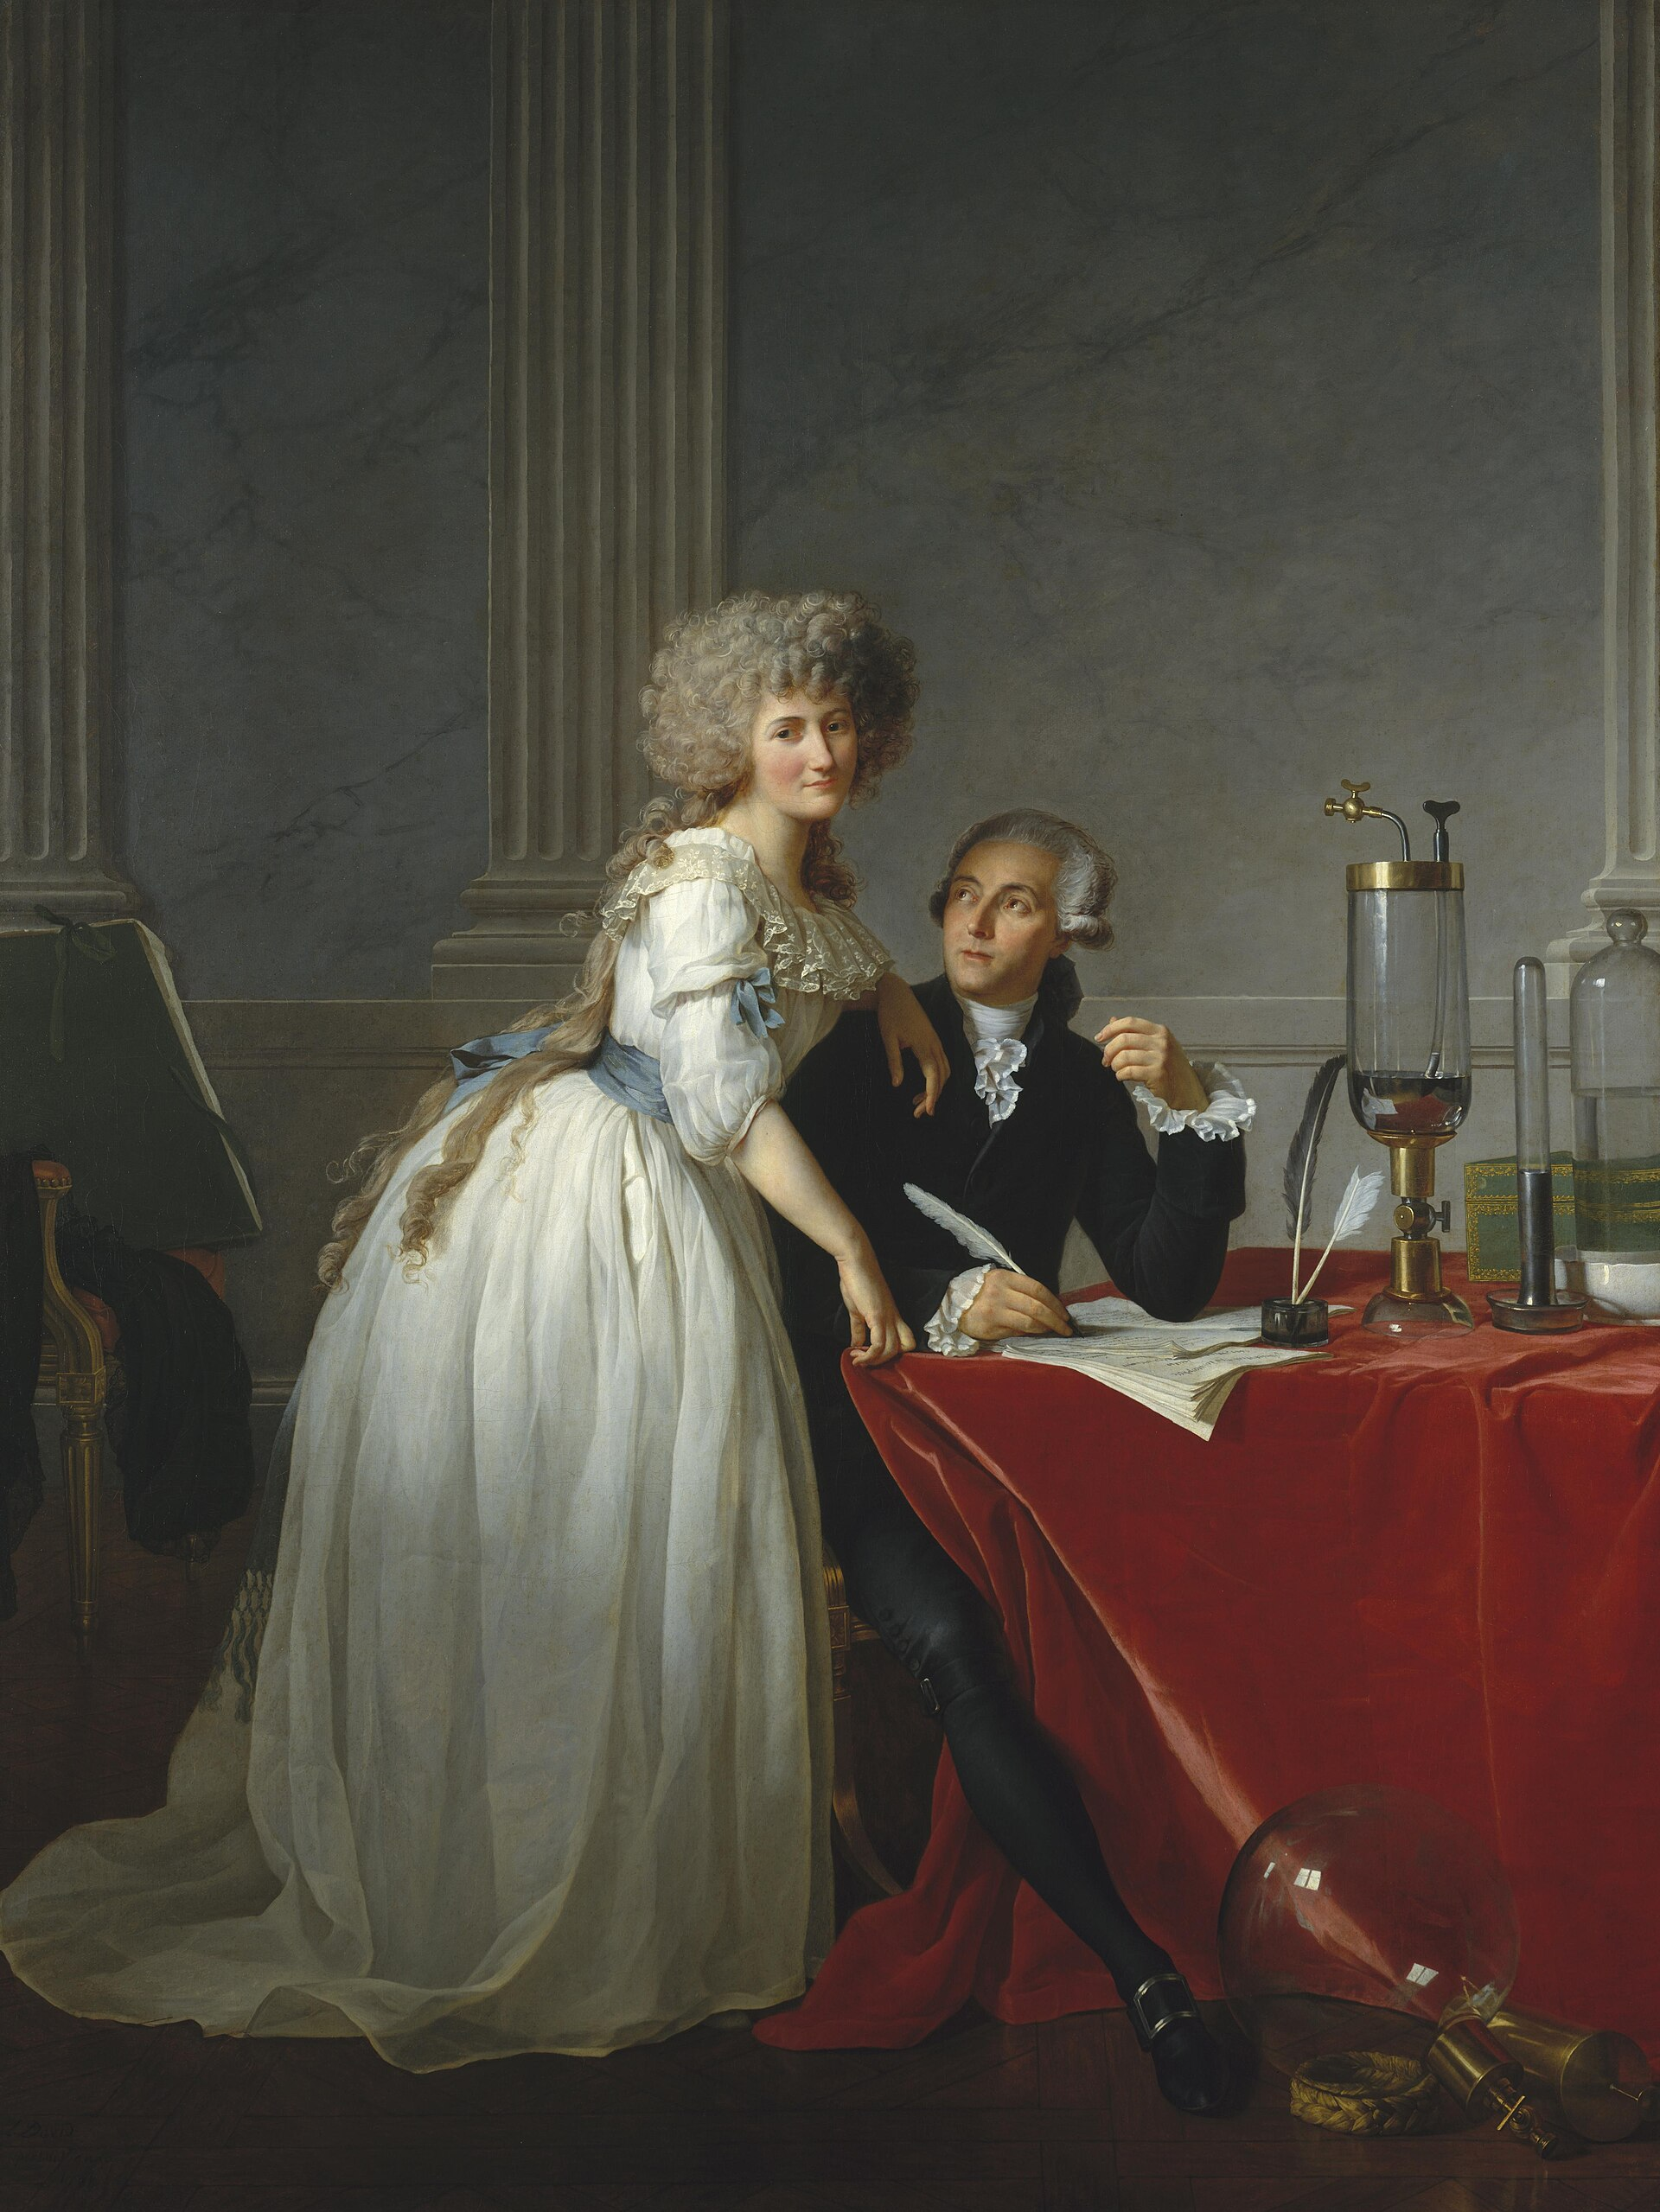
\includegraphics[width=0.3\linewidth]{images/book1/lavoisier.jpg}

{\small Antoine-Laurent Lavoisier en Marie-Anne Paulze Lavoisier, door
Jacques-Louis David, 1788.}
\end{omfigure}

\section{Waarom massa behouden blijft}

\begin{proposition}[Atomen blijven behouden, dus massa blijft behouden]\label{prop:g8:balanced-equations:why}
Bij een reactie worden de \omterm{def:g7:atoms-and-molecules:atom}{atomen} alleen herschikt: elk \omterm{def:g7:atoms-and-molecules:atom}{atoom} van de
\omterm{def:g7:chemical-reactions:reactant}{beginstoffen} vind je terug in de \omterm{def:g7:chemical-reactions:reactant}{reactieproducten}. Elk \omterm{def:g7:atoms-and-molecules:atom}{atoom} houdt zijn
eigen massa. De totale massa kan dus niet veranderen.
\end{proposition}

\begin{example}[IJzer dat zwaarder wordt]\label{ex:g8:balanced-equations:iron}
Staalwol die in een open schaaltje op een balans verbrandt, wordt
zwaarder: de ijzeratomen hebben zich verbonden met zuurstofatomen uit de
\omterm{def:g4:air-a-mixture-of-gases:air}{lucht}, en het gevormde ijzeroxide weegt evenveel als het ijzer plus die
zuurstof. Verbrand je het in een afgesloten pot met \omterm{def:g4:air-a-mixture-of-gases:air}{lucht} op de balans,
dan verandert de massa van het geheel niet: de zuurstof zat al in de
pot.
\end{example}

\section{De reactievergelijking}

\begin{definition}[Reactievergelijking]\label{def:g8:balanced-equations:equation}
Een \emph{reactievergelijking}\index{reactievergelijking} schrijft een
reactie op met formules: links de formules van de \omterm{def:g7:chemical-reactions:reactant}{beginstoffen},
verbonden door $+$, dan een pijl, en rechts de formules van de
\omterm{def:g7:chemical-reactions:reactant}{reactieproducten}. Voor elke formule mag een getal staan. De vergelijking
is een \emph{kloppende reactievergelijking}\index{kloppende reactievergelijking}
als elke soort \omterm{def:g7:atoms-and-molecules:atom}{atoom} aan beide kanten even vaak voorkomt.
\end{definition}

\begin{definition}[Coëfficiënt]\label{def:g8:balanced-equations:coefficient}
Het getal dat in een \omterm{def:g8:balanced-equations:equation}{reactievergelijking} vóór een formule staat, is de
\emph{coëfficiënt}\index{coëfficiënt}: hij telt de \omterm{def:g7:atoms-and-molecules:molecule}{moleculen} (of
andere deeltjes) van die stof die meedoen. Een coëfficiënt 1 schrijf je
niet.
\end{definition}

\begin{notation}[Toestandsaanduidingen]\label{not:g8:balanced-equations:states}
Een letter tussen haakjes na een formule kan de toestand aangeven:
(s) vast, (l) vloeibaar, (g) gas. Zo is \ce{H2O(l)} vloeibaar water en
\ce{H2O(g)} waterdamp.
\end{notation}

\begin{example}[Een reactievergelijking lezen]\label{ex:g8:balanced-equations:read}
\[
  \ce{CH4(g) + 2O2(g) -> CO2(g) + 2H2O(l)}
\]
lees je als: één methaanmolecuul en twee zuurstofmoleculen reageren tot
één koolstofdioxidemolecuul en twee watermoleculen. Links: 1 C, 4 H, 4 O.
Rechts: 1 C, 4 H, $2 + 2 = 4$ O. De vergelijking klopt.
\end{example}

\begin{omfigure}
\begin{tikzpicture}[font=\small]
  \begin{scope}[every node/.style={font=\Large, inner sep=2pt}]
    \node (a) at (0,0) {\ce{CH4}};
    \node (p1) at (0.95,0) {$+$};
    \node (b) at (1.9,0) {\ce{2O2}};
    \node (arr) at (3.35,0) {$\longrightarrow$};
    \node (c) at (4.8,0) {\ce{CO2}};
    \node (p2) at (5.75,0) {$+$};
    \node (d) at (6.8,0) {\ce{2H2O}};
  \end{scope}
  \draw[thick, omDef] ([yshift=-2pt]a.south west) -- ++(0,-0.15) -| ([yshift=-2pt]b.south east);
  \node[below=8pt, text=black] at ($(a.south)!0.5!(b.south)$) {beginstoffen};
  \draw[thick, omProp] ([yshift=-2pt]c.south west) -- ++(0,-0.15) -| ([yshift=-2pt]d.south east);
  \node[below=8pt, text=black] at ($(c.south)!0.5!(d.south)$) {reactieproducten};
  \node[above=6pt of arr, font=\small] {``reageren tot''};
  \node[anchor=north west, align=left, draw=black!35, rounded corners=2pt,
    font=\small, inner sep=4pt] at (-0.3,-1.25)
    {In \ce{2O2}: de grote 2 ervoor is de \textbf{coëfficiënt} (twee moleculen);\\
     de kleine 2 onder de regel is de \textbf{index} (twee atomen per molecuul).};
\end{tikzpicture}

{\small De onderdelen van een \omterm{def:g8:balanced-equations:equation}{reactievergelijking}.}
\end{omfigure}

\section{Een reactievergelijking kloppend maken}

\begin{method}[Een reactievergelijking kloppend maken]\label{met:g8:balanced-equations:balance}
\begin{enumerate}
  \item Schrijf de juiste formules van de \omterm{def:g7:chemical-reactions:reactant}{beginstoffen} en de
        \omterm{def:g7:chemical-reactions:reactant}{reactieproducten} op. Verander een formule daarna nooit meer: als
        je \ce{H2O} in \ce{H2O2} verandert, beschrijf je een andere stof.
  \item Tel aan elke kant de \omterm{def:g7:atoms-and-molecules:atom}{atomen} van elke soort.
  \item Maak één soort \omterm{def:g7:atoms-and-molecules:atom}{atoom} tegelijk kloppend met \omterm{def:g8:balanced-equations:coefficient}{coëfficiënten}; begin
        met de \omterm{def:g7:atoms-and-molecules:atom}{atomen} die aan elke kant in maar één formule voorkomen, en
        bewaar waterstof en zuurstof voor het laatst.
  \item Tel opnieuw; herhaal tot elke soort \omterm{def:g7:atoms-and-molecules:atom}{atoom} klopt.
  \item Gebruik de kleinste gehele getallen.
\end{enumerate}
\end{method}

\begin{example}[Waterstof en zuurstof]\label{ex:g8:balanced-equations:water}
Niet kloppend: \ce{H2 + O2 -> H2O} % ce-unbalanced-ok (the skeleton)
heeft links 2 O en rechts 1. Zet 2 voor \ce{H2O}: nu staan er rechts
4 H, dus zet 2 voor \ce{H2}:
\[
  \ce{2H2 + O2 -> 2H2O}.
\]
Controle: aan elke kant 4 H en 2 O.
\end{example}

\begin{example}[IJzer dat in zuurstof verbrandt]\label{ex:g8:balanced-equations:iron-oxide}
IJzer en zuurstof geven het ijzeroxide \ce{Fe2O3}. Zuurstof: links 2,
rechts 3; het kleinste gemeenschappelijke getal is 6, dus 3 \ce{O2} en
2 \ce{Fe2O3}. Dan staan er rechts 4 Fe, dus links ook 4 Fe:
\[
  \ce{4Fe + 3O2 -> 2Fe2O3}.
\]
\end{example}

\begin{omfigure}
\begin{tikzpicture}[font=\small]
  % 2 H2
  \foreach \y in {0.45,-0.45} {
    \node[aH] (a) at (0,\y) {}; \node[aH] (b) at (0.45,\y) {};
    \begin{scope}[on background layer]\draw[bond] (a.center) -- (b.center);\end{scope}}
  \node at (1.05,0) {$+$};
  \node[aO] (a) at (1.6,0) {}; \node[aO] (b) at (2.25,0) {};
  \begin{scope}[on background layer]
    \draw[bond, line width=1.1pt] ([yshift=1.6pt]a.center) -- ([yshift=1.6pt]b.center);
    \draw[bond, line width=1.1pt] ([yshift=-1.6pt]a.center) -- ([yshift=-1.6pt]b.center);
  \end{scope}
  \draw[->, thick, omProp] (2.9,0) -- (3.9,0);
  \foreach \y in {0.5,-0.5} {
    \node[aO] (o) at (4.9,\y+0.12) {};
    \node[aH] (p) at (4.35,\y-0.28) {}; \node[aH] (q) at (5.45,\y-0.28) {};
    \begin{scope}[on background layer]
      \draw[bond] (o.center) -- (p.center); \draw[bond] (o.center) -- (q.center);
    \end{scope}}
  \node[align=center, font=\footnotesize] at (1.1,-1.35) {4 H, 2 O};
  \node[align=center, font=\footnotesize] at (4.9,-1.35) {4 H, 2 O};
  \node[font=\small] at (2.7,-2.0) {\ce{2H2 + O2 -> 2H2O}};
\end{tikzpicture}

{\small De \omterm{def:g8:balanced-equations:equation}{kloppende reactievergelijking} van de \omterm{def:g4:what-a-fire-needs:burning}{verbranding} van
waterstof, getekend met modellen: twee waterstofmoleculen en één
zuurstofmolecuul geven twee watermoleculen.}
\end{omfigure}

\section{Een reactievergelijking in moleculen lezen}


\begin{proposition}[Wat een kloppende reactievergelijking zegt]\label{prop:g8:balanced-equations:molecules}
De \omterm{def:g8:balanced-equations:coefficient}{coëfficiënten} van een \omterm{def:g8:balanced-equations:equation}{kloppende reactievergelijking} geven de
verhoudingen waarin de deeltjes reageren en gevormd worden. Luidt de
vergelijking \ce{2H2 + O2 -> 2H2O}, dan reageren 200 waterstofmoleculen
met 100 zuurstofmoleculen tot 200 watermoleculen; een miljoen
zuurstofmoleculen hebben twee miljoen waterstofmoleculen nodig.
\end{proposition}

\begin{example}[Propaan in een kampeerbrander]\label{ex:g8:balanced-equations:propane}
Propaan, \ce{C3H8}, verbrandt in zuurstof tot koolstofdioxide en water.
Eerst koolstof: 3 C, dus 3 \ce{CO2}. Waterstof: 8 H, dus 4 \ce{H2O}.
Zuurstof rechts: $3 \times 2 + 4 = 10$ O, dus 5 \ce{O2}:
\[
  \ce{C3H8 + 5O2 -> 3CO2 + 4H2O}.
\]
Elk propaanmolecuul heeft vijf zuurstofmoleculen nodig.
\end{example}

\section{Oefeningen}

\begin{exercise}[$\star$]\label{exo:g8:balanced-equations:1}
Formuleer de wet van \omterm{def:g8:balanced-equations:conservation}{behoud van massa}.
\end{exercise}

\begin{exercise}[$\star$]\label{exo:g8:balanced-equations:2}
Wat is in \ce{3CO2} de \omterm{def:g8:balanced-equations:coefficient}{coëfficiënt}? Hoeveel koolstofatomen en hoeveel
zuurstofatomen stelt het voor?
\end{exercise}

\begin{exercise}[$\star$]\label{exo:g8:balanced-equations:3}
Klopt \ce{C + O2 -> CO2}? Tel de \omterm{def:g7:atoms-and-molecules:atom}{atomen} om het te controleren.
\end{exercise}

\begin{exercise}[$\star$]\label{exo:g8:balanced-equations:4}
Maak \ce{Mg + O2 -> MgO} kloppend. % ce-unbalanced-ok (to balance)
\end{exercise}

\begin{exercise}[$\star\star$]\label{exo:g8:balanced-equations:5}
Maak \ce{N2 + H2 -> NH3} kloppend, de reactie waarmee ammoniak gemaakt wordt. % ce-unbalanced-ok (to balance)
\end{exercise}

\begin{exercise}[$\star\star$]\label{exo:g8:balanced-equations:6}
Er verbrandt \qty{12}{g} koolstof volledig, en daarbij ontstaat
\qty{44}{g} koolstofdioxide. Hoeveel zuurstof is er verbruikt?
\end{exercise}

\begin{exercise}[$\star\star$]\label{exo:g8:balanced-equations:7}
Kijk naar de figuur van de twee kolven op balansen. Waarom daalt de
aflezing van de open kolf? Is er massa vernietigd?
\end{exercise}

\begin{exercise}[$\star\star$]\label{exo:g8:balanced-equations:8}
Maak \ce{CH4 + O2 -> CO2 + H2O} stap voor stap kloppend, en zeg bij % ce-unbalanced-ok (to balance)
elke stap welk \omterm{def:g7:atoms-and-molecules:atom}{atoom} je kloppend maakt.
\end{exercise}

\begin{exercise}[$\star\star$]\label{exo:g8:balanced-equations:9}
Een leerling maakt \ce{H2 + O2 -> H2O} kloppend door \ce{H2 + O2 -> H2O2} te schrijven. % ce-unbalanced-ok (the student's start)
Waarom is dat fout?
\end{exercise}

\begin{exercise}[$\star\star$]\label{exo:g8:balanced-equations:10}
Hoeveel zuurstofmoleculen zijn er volgens \ce{C3H8 + 5O2 -> 3CO2 + 4H2O}
nodig om 20 propaanmoleculen te \omterm{def:g4:what-a-fire-needs:burning}{verbranden}? Hoeveel watermoleculen
worden er gevormd?
\end{exercise}

\begin{exercise}[$\star\star\star$]\label{exo:g8:balanced-equations:11}
Maak \ce{C2H6 + O2 -> CO2 + H2O} kloppend, de \omterm{def:g4:what-a-fire-needs:burning}{verbranding} van ethaan. % ce-unbalanced-ok (to balance)
(Tip: probeer het ethaan te verdubbelen.)
\end{exercise}

\begin{exercise}[$\star\star\star$]\label{exo:g8:balanced-equations:12}
Een kaars van \qty{20.0}{g} brandt in een afgesloten glazen doos vol
\omterm{def:g4:air-a-mixture-of-gases:air}{lucht}, die op een balans staat die in totaal \qty{850.0}{g} aanwijst.
Als de vlam uitgaat, weegt de kaars \qty{19.6}{g}. Wat wijst de balans
aan? Leg uit.
\end{exercise}

\section{Probleem: Staalwol in een afgesloten pot}

\begin{problem}[{Weekendprobleem --- ijzer dat verbrandt, een balans die
niet beweegt, en de zuurstof die uit de lucht wordt gehaald}]
\label{pb:g8:balanced-equations:1}
In een laboratorium verbrandt een docent staalwol, die bijna zuiver ijzer
is, op twee manieren. Eerst wordt een plukje in een open schaaltje op
een balans verbrand: de aflezing stijgt. Daarna wordt een plukje van
\qty{0.28}{g}, aangestoken met een elektrische vonk, verbrand in een
gesloten pot met \omterm{def:g4:air-a-mixture-of-gases:air}{lucht} die op de balans staat: de aflezing verandert
niet. De pot bevat ongeveer \qty{0.5}{g} zuurstof. IJzer dat in zuurstof
verbrandt, vormt het ijzeroxide \ce{Fe2O3}; met minder zuurstof kan het
ook \ce{Fe3O4} vormen.

\medskip
\noindent\textbf{Deel I --- Twee wegingen.}
\begin{enumerate}
  \item In het open schaaltje neemt de massa toe. Waar komt de extra
        massa vandaan?
  \item In de gesloten pot verandert de massa niet. Leg uit.
  \item Formuleer de wet die deze twee wegingen illustreren.
\end{enumerate}

\medskip
\noindent\textbf{Deel II --- Twee \omterm{def:g8:balanced-equations:equation}{reactievergelijkingen}.}
\begin{enumerate}[resume]
  \item Maak de \omterm{def:g8:balanced-equations:equation}{reactievergelijking} \ce{Fe + O2 -> Fe2O3} kloppend. % ce-unbalanced-ok (to balance)
  \item Maak de \omterm{def:g8:balanced-equations:equation}{reactievergelijking} \ce{Fe + O2 -> Fe3O4} kloppend. % ce-unbalanced-ok (to balance)
  \item Controleer de eerste vergelijking door aan elke kant de \omterm{def:g7:atoms-and-molecules:atom}{atomen}
        van elke soort te tellen.
  \item Hoeveel zuurstofmoleculen reageren er volgens de eerste
        vergelijking met 400 ijzeratomen?
\end{enumerate}

\medskip
\noindent\textbf{Deel III --- Massa's.}
In \ce{Fe2O3} is elke \qty{7}{g} ijzer verbonden met \qty{3}{g}
zuurstof. Het plukje van \qty{0.28}{g} verbrandt volledig tot \ce{Fe2O3}.
\begin{enumerate}[resume]
  \item Hoeveel zuurstof verbindt zich met \qty{0.28}{g} ijzer?
  \item Wat is de massa van het gevormde ijzeroxide?
  \item Was er genoeg zuurstof in de pot? Leg uit.
  \item Na het afkoelen wordt de pot geopend, en er stroomt \omterm{def:g4:air-a-mixture-of-gases:air}{lucht} naar
        binnen. Leg uit waarom, en zeg hoe de aflezing van de balans dan
        verandert.
  \item Bereken de massa zuurstof die de brandende staalwol uit de \omterm{def:g4:air-a-mixture-of-gases:air}{lucht}
        in de pot heeft gehaald.
\end{enumerate}
\end{problem}
